\section{Das Das Rosenblatt-Perzeptron}

In Abschnitt~\ref{mcp-summary} haben wir geschlossen, dass ein MCP-Netz nur durch vorhergehende Analyse der Aufgabe und Anpassung der Topologie von Außen zur Lösung einer Aufgabe imstande ist.
\textit{Donald Hebbs} Erkenntnisse\footnote{
    s. \ref{appendix:hebb}
} führt kurz vor Beginn der 60er Jahre zu einem Modell, das in der Lage ist, sich selbst anzupassen.


\subsection{Das Perzeptron - ein linearer Klassifizierer}

Bereits 1954 wurden Versuche unternommen, lernfähige neuronale Netze zu modellieren~\cite[24]{Ros62}\footnote{
    Rosenblatt verweist hier auf~\cite{FC54}
}.
Erst 1958 schafft es ein Modell, eine Sensation\footnote{
    In der Presse publikumswirksam, aber wenig vertrauenserweckend: ``Frankenstein Monster Designed by Navy Robot That Thinks``~\cite[v]{Ros62}. Vgl. dazu aktuelle Schlagzeilen der hiesigen Boulevardpresse zum Thema KI. bild.de titelt: ``Übernehmen Computer die Weltherrschaft?`` (\url{https://www.bild.de/news/ausland/news-ausland/experten-warnen-ki-so-gefaehrlich-wie-pandemien-und-atomkrieg-84130180.bild.html}, abgerufen 27.08.2023) als Reaktion auf ``Statement on AI Risk`` des \textit{Center for AI Safety}, in dem zahlreiche Wissenschaftler zur Vorsicht beim Umgang, Einsatz und Forschung von KI mahnen. Im Wortlaut: ``Mitigating the risk of extinction from AI should be a global priority alongside other societal-scale risks such as pandemics and nuclear war.`` (\url{https://www.safe.ai/statement-on-ai-risk}, abgerufen 27.08.2023)
} auszulösen: Das \textbf{Perceptron} (im folgenden ``Perzeptron``)~\cite[89]{AR88}\footnote{
    s. auch ``Interest in connectionist networks revivied dramatically in 1962 with the publication of Frank Rosenblatt's book \textit{Principles of Neurodynamics}, [...]``~\cite[xi, Hervorhebung i.O.]{MP88}
}.
1957 beschreibt es sein Schöpfer \textit{Frank Rosenblatt} (1928 - 1971) in~\cite{Ros57}\footnote{
    s. \ref{appendix:perzeptron}
} als Teil eines internen Forschungsprojektes des \textit{Cornell Aeronautical Labors}\footnote{
    Die Forschungseinrichtung gehörte von 1946 bis 1972 zu der Cornell Universität (\url{https://www.cornell.edu}; ab 1972 gehörte die Forschungseinrichtung dann zu der Calspan Corporation, \url{https://calspan.com}, beides abgerufen 18.08.2023)
}, an der Rosenblatt 1950 seinen A.B und 1956 seinen Ph.D. gemacht hatte, und an der er bis zu seinem Lebensende\footnote{
    1971 durch einen Bootsunfall; \url{https://ecommons.cornell.edu/items/91237274-dd25-4969-99cb-8758ca05cec9}, abgerufen 19.09.2023
} als Psychologe und Neurobiologe forschen und lehren wird.


\subsection{Das Modell}

Rosenblatt definiert das Perzeptron wie folgt\footnote{
    Ausführliche Definitionen aller Zustände, Signale und Funktionen in~\cite[79 - 94]{Ros62}
}:

\blockquote[{\cite[83 ``DEFINITION 17`` (Hervorhebung i.O.)]{Ros62}}]{
    A \underline{perceptron} is a network of S, A, and R units with a variable interaction matrix \textit{V} which depends on the
    sequence of past activity states of the network.
}

Für die \textbf{A}-Units wird definiert:

\blockquote[{\cite[81  ``DEFINITION 9`` (Hervorhebung i.O.)]{Ros62}}]{
    A \underline{simple A-unit} is a logical decision element, which
    generates an output signal if the algebraic sum of its
    input signals, $\alpha_i$ , is equal or greater than a threshold
    quantity, $\Theta > 0$. The output signal $a^*_i$ is equal to $+1$ if $\alpha_i \geq \Theta$ and $0$ otherwise. If $a^*_i = +1$,
    the unit is said to be \underline{active}.
}


Ähnlichkeiten zu der in Abschnitt~\ref{mcp-inputactivfunc} beschriebenen Aktivierungsfunktion sind durchaus erkennbar.
Rosenblatt selber weist darauf hin, dass er sein Modell direkt von dem von McCulloch und Pitts eingeführten Modell ableitet\footnote{
    vgl. auch ``Ein \texit{einfaches Perzeptron} ist eine McCulloch-Pitts-Zelle, die ihre Eingabe gewichtet berechnet.`` in~\cite[57, ``Definition 3.1`` (Hervorhebungen i.O.)]{Roj93}
}. Darüber hinaus weist er auch auf Einflüsse von Hebb und von Neumann hin~\cite[5]{Ros62}.\\


\textit{Rojas} schreibt in~\cite[51]{Roj93}, dass das klassische Rosenblatt-Perzeptron in einem Netz von Eingabe- und Ausgabe-Knoten gewichtete Verbindungen nutzt - die Knoten selber sind Schwellenwertelemente, Verbindungen werden stochastisch ermittelt.
Er weist dort ausserdem darauf hin, dass nach Rosenblatts Veröffentlichung sein Modell analysiert und verfeinert wurde, u. a. von \textit{Minsky und Papert} in~\cite{MP88}, die wie folgt definieren:

\blockquote[{~\cite[12, Hervorhebung i.O.]{MP88}}]{
    A \underline{perceptron} is a device capable of computing all predicates which are linear in some given set $\Phi$ of partial predicates.
}

Prädikate sind hier Verbindungen zu den Eingabesignalen, die einen Wahrheitswert $0$ oder $1$ basierend auf der Eingabe $X$ berechnen.
Die Ausgabe der Prädikate werden individuell gewichtet und an die Zelle weitergeleitet, die die Aktivierungsfunktion implementiert (vgl.~\cite[52 f.]{Roj93} und~\cite[8-12]{MP88}).


\begin{figure}[h]
    \centering
    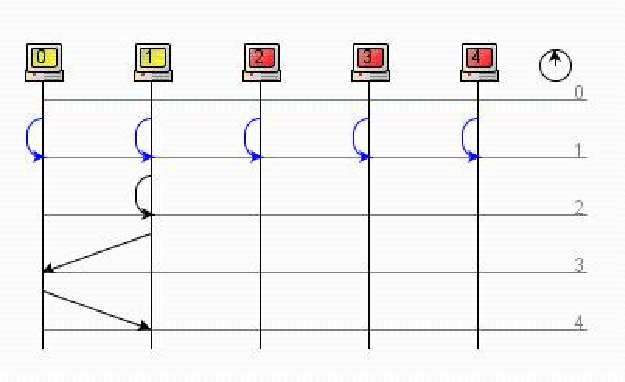
\includegraphics{images/p1ReadSeq.pdf}
    \caption{Schematische Darstellung der Eingabesignale, Prädikate, Gewichte und Schwellenwertzelle nach~\cite[53 Abb. 3.2]{Roj93}}
    \label{fig-perctheda}
\end{figure}


Die Eingabefunktion setzt sich dann wie Gleichung~\ref{eq:gl-mcpinpfunc} aus der Summe der Produkte der Prädikate $P_i \in \Phi$ (wobei $P_i(X) \in \{0, 1\}$) und den Gewichten $w_i \in \R$ der Verbindungen zusammen (s. Gleichung~\ref{eq:gl-rpinput}), und die Aktivierungsfunktion (s. Gleichung~\ref{eq:gl-rpact}) ist wieder eine Treppenfunktion mit dem reellen Schwellenwert $\Theta$:

\begin{equation}
g:= g(X) = \sum^n_{i=1} P_i(X) w_i
\label{eq:gl-rpinput}
\end{equation}

\begin{equation}
    f:= f(x) = f(g(X)) = \begin{cases}
                          1 \text{ falls } x >= \Theta \\
                          0 \text{ falls } x < \Theta
\end{cases}
\label{eq:gl-rpact}
\end{equation}

\noindent
\textit{Minsky und Papert} weisen in ihrer Definition des Perzeptrons auf eine besondere Voraussetzung hin, die Thema des nächsten Abschnitts wird.

\subsection{Lineare Trennbarkeit}
Mit Gleichung~\ref{eq:gl-rpact} folgt für eine Eingabe, dass sie entweder eine $0$ oder $1$ als Ausgabe erzeugt.
Wir haben es hier also wieder mit einem binären Wertebereich zu tun, den wir auch als zwei unterschiedliche Klassen [RN09:812, Abs. 2] verstehen können: Eingabedaten können somit einer der beiden Klassen zugeordnet werden.
Im Folgenden wollen wir die Zusammenhänge geometrisch darstellen.
Der Einfachheit halber beschränken wir uns hierzu auf den zweidimensionalen Raum $\R_+^2$ und betrachten hier die \textit{1. Winkelhalbierende} im 1. Quadrant des kartesischen Koordinatensystems.
Die zugehörige \textit{Gerade} $L$ ist

\begin{equation}
L = \{(x_1, x_2) \in \R_+^2: x_1 = x_2\}
\end{equation}


\begin{figure}[h]
    \centering
    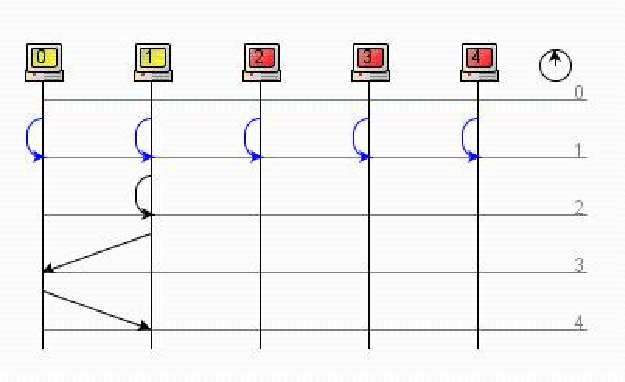
\includegraphics{images/p1ReadSeq.pdf}
    \caption{Winkelhalbierende im kartesischen Koordinatensystem}
    \label{fig-winkelhalbierende}
\end{figure}

Für beliebige Punkte $(x_1, x_2) \in \R_+^2$ gilt offensichtlich

\begin{equation}
x_1 - x_2 \begin{cases}
               > 0 \text{ falls } x_1 > x_2 \\
               = 0 \text{ falls } x_1 = x_2 \\
               < 0 \text{ falls } x_1 < x_2
\end{cases}
\end{equation}

Die \textit{Gerade} $L$ repräsentiert eine \textit{Hyperebene} in $\R_+^2$~\cite[81, Definition 2.3]{BHW+12}.
Punkte, die nicht zu dieser Hyperebene gehören, liegen in dem Fall $\R_+^2$ in zwei unterschiedlichen \textit{Halbräumen}\footnote{
    Renze, John; Uznanski, Dan; and Weisstein, Eric W. ``Half-Plane.`` From MathWorld--A Wolfram Web Resource. \url{https://mathworld.wolfram.com/Half-Plane.html} (abgerufen 21.08.2023)
}.
Die Halbräume und deren Trennung wird greifbarer durch die geometrische Darstellung in Abbildung~\ref{fig-halbraeume}.
Wir können feststellen, dass


\begin{itemize}
    \item Punkte, die $x_1 - x_2 > 0$ erfüllen (im folgenden $M_-$) in dem Halbrum \textit{unter} der durch $L$ beschriebenen Gerade liegen
    \item Punkte, für die  $x_1 - x_2 < 0$ gilt (im folgenden $M_+$) \textit{über} der durch $L$ beschriebenen Gerade liegen
    \item Punkte mit $x_1 - x_2 = 0$ \textit{auf} der Geraden liegen (im folgenden $\subset M_-$\footnote{
        Wenn die Hyperebene selbst im Halbraum enthalten ist, spricht man von einem \textit{abgeschlossenen Halbraum}. (\url{https://de.wikipedia.org/wiki/Halbraum}, abgerufen 22.08.2023)
    })
\end{itemize}


\begin{figure}[h]
    \centering
    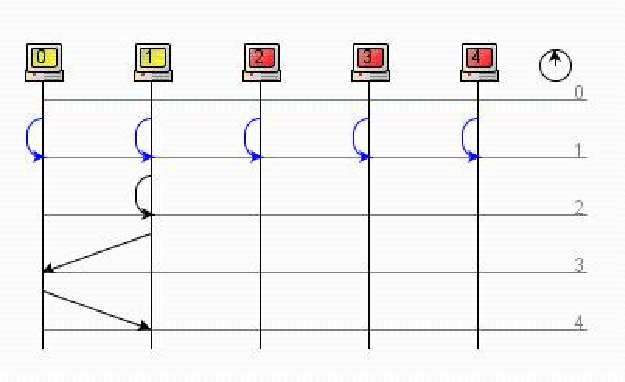
\includegraphics{images/p1ReadSeq.pdf}
    \caption{Skizzierung der durch die 1. Winkelhalbierende entstandenen Halbräume. Die Mengen $M_-$ und $M_+$ sind linear separierbar, die Gleichung für die \textit{Trenngerade} hierzu lautet $x_1 - x_2 = 0$}
    \label{fig-halbraeume}
\end{figure}

Formal ausgedrückt bedeutet das, dass $M_+$ und $M_-$ \textit{linear separabel} sind. Nach \textit{Rojas} lautet die Definition für \textit{Lineare Trennbarkeit}:

\begin{definition}\footnote{
    \cite[60, ``Definition 3.2`` (Hervorhebungen i.O., Nummerierung eigene)]{Roj93}
}

Zwei Mengen \textit{A} und \textit{B} von Punkten in einem \textit{n}-dimensionalen Raum sind \textit{linear trennbar}, falls \textit{n}+1 reelle Zahlen $w_1, ... , w_{n+1}$ existieren, so daß für jeden Punkt $x_1, ... , x_n \in A$ gilt

\begin{equation}
\sum^n_{i=1} w_ix_i \geq w_{n+1}
\label{eq:gl-defhalbraum-gl1}
\end{equation}

und für jeden Punkt $x_1, ... , x_n \in B$

\begin{equation}
    \sum^n_{i=1} w_ix_i < w_{n+1}
\label{eq:gl-defhalbraum-gl2}
\end{equation}
\label{def-halbraum}
\end{definition}


\noindent
Für unser Beispiel mit den oben eingeführten Mengen $M_- = \{(x_1, x_2) \in  \mathbb{R}_+^2: x_1 \geq x_2\}$ und $M_+=\{(x_1, x_2) \in  \mathbb{R}_+^2: x_1 < x_2\}$ in $ \mathbb{R}_+^2$ wählen wir $w_1 = -1, w_2 = 1, w_3 = 0$.
Dass diese Mengen nach Definition~\ref{def-halbraum} linear separabel sind, lässt sich leicht anhand einer Fallunterscheidung nachweisen:

\begin{enumerate}
    \item Fall $x_1 = x_2$: Es gilt $w_1x_1 + w_2x_2 = w_1x_1 + w_2x_1 = -x_1 + x_1 = w_3 = 0$. Mit $0 \geq 0$ ist somit Gleichung~\ref{eq:gl-defhalbraum-gl1} erfüllt.
    \item Fall $x_1 < x_2$: Es gilt $w_1x_1 = -x_1$. Addition von $w_1x_1$ auf beiden Seiten von $x_2 > x_1$ liefert $x_2 + (-x_1) = w_2x_2 + w_1x_1 > 0 = w_3$ und erfüllt Gleichung~\ref{eq:gl-defhalbraum-gl1}.
    \item Fall $x_1 > x_2$: Es gilt wieder $w_1x_1 = -x_1$. Addition auf beiden Seiten von $x_1 > x_2$ liefert $w_3 = 0 > x_2 + (-x_1) = w_2x_2 + w_1x_1$ und erfüllt Gleichung~\ref{eq:gl-defhalbraum-gl2}.
\end{enumerate}


\noindent
Die von \textit{Ertel} formulierte Definition für ein Perzeptron wollen wir für die weiteren Betrachtungen übernehmen\footnote{
    \cite[212, ``Definition 8.3``, Hervorhebungen i.O.]{Ert21a}
}:

\begin{definition}
\noindent
Sei $w = (w_1, ..., w_n) \in  \mathbb{R}^n$ ein Gewichtsvektor und $x \in  \mathbb{R}^n$ ein Eingabevektor. Ein \textbf{Perzeptron} stellt eine Funktion $P:  \mathbb{R}^n \to \{0, 1\}$ mit

\begin{equation}
P(x) = \begin{cases}
            1 \text{ falls } wx = \sum^n_{i=1} w_ix_i >0 \\
            0 \text{sonst}
\end{cases}
\end{equation}
\noindent
dar.

\end{definition}

\subsection{Die Lernregel}\label{sec-lernregel}

Die Eigenschaft linearer Trennbarkeit von Daten ist eine wesentliche Voraussetzung dafür, dass ein Perzeptron \textit{konvergiert}: Die \textit{Lernregel} des Perzeptrons passt während der Laufzeit die Gewichte $w_1 ... w_n$ solange an, bis sie - eingesetzt in eine lineare Gleichung~\cite[311]{Ert21b} - die $n$-dimensionalen Daten entsprechend Definition~\ref{eq:gl-rpact} \textit{klassifizieren} kann.
Aus diesem Grund wird das Perzeptron auch \textbf{linearer Klassifizierer} genannt (vgl.~\cite[210-216]{Ert21a}).

Das Perzeptron \textbf{lernt} diese Gewichte zunächst durch \textit{Traningsdaten}\footnote{
    ``supervised learning``: überwachtes lernen; vgl. [RN09:811, ``18.2 Überwachtes Lernen``] sowie [Fau94:15]. \textit{Arbib et al.} weisen darauf hin, dass \textit{überwachtes Lernen} mit dem Perzeptron eingeführt wurde: ``Supervised learning adjusts the weights in an attempt to respond to explicit error signals provided by a “teacher,” which may be external, or another network in the same “brain.” This model was introduced in the perceptron model, [...].``~\cite[30]{Arb03}
}.
Jeder Eintrag dieser Trainingsdaten ist einer erwarteten Ausgabe zugeordnet. Der Algorithmus besteht aus folgenden Schritten (vgl.~\cite[65]{RM87} sowie [RN09 S. 842]):



\begin{enumerate}
    \item Wähle einen Datensatz und berechne die Ausgabe
    \item Wenn die Ausgabe $1$ ist, obwohl sie $0$ sein sollte (Fehler\footnote{
    Der \textbf{Fehler} ist hierbei die Differenz von $\text{erwartete Ausgabe}$ und $\text{tatsächliche Ausgabe}$.
    } $=-1$), verringere die Gewichte
    \item Wenn die Ausgabe $0$ ist, obwohl sie $1$ sein sollte  (Fehler $=1$), erhöhe die Gewichte
    \item Wenn die Ausgabe korrekt ist, passe die Gewichte nicht an
\end{enumerate}

\noindent
Die Beziehung zu der Hebbschen Lernregel formulieren \textit{Arbib et al.}\footnote{
    vgl. hierzu auch _Rosenblatt_ : ``[ein Perzeptron hat] a tendency to develop 'cell assemblies' (in Hebb's sense), and these cell-assemblies tend to rival one another for dominance at all times.``~\cite[464]{Ros62}
}:

\blockquote[{\cite[20]{Arb03}}]{
    The best-known perceptron learning rule strengthens an active synapse if the efferent neuron fails to fire when it should have fired, and weakens an active synapse if the neuron fires when it should not have done so.
}

\noindent
Die Schritte werden so lange durchlaufen, bis für alle Trainingsdaten die Ausgabe korrekt ist, oder eine maximale Anzahl von Trainingsläufen erreicht wurde.
Einen Trainingslauf nennt man dabei \textit{Epoche} [Fau94:436, ``Training epoch``].
Sind die Trainingsdaten linear separabel, \textit{konvergiert}\footnote{
    ``iterative training processes converge if the weight updates reach equilibrium (stop changing)`` [Fau94:425, ``Convergence``]
} das Perzeptron nach einer endlichen Zahl von Epochen~\cite[164]{MP88}\footnote{
    Das Konvergenz-Theorem besagt: ``if a linear separation exists, the perceptron error-correction scheme will find it.``~\cite[20]{Arb03}] Beweise führen~\cite[111 ff.]{Ros62}, \cite[168 ff.]{MP88} sowie \cite{Nov62}.
}, und ist danach in der Lage zu \textit{generalisieren}~\cite[202]{Ert21a}.\\

Da wir in unserem Beispiel nur Daten betrachtet haben, die durch eine Gerade durch den Ursprung ($(0,0)$) getrennt sind, brauchen wir noch eine Möglichkeit, die $x_2$-Koordinate der Trenngerade anzupassen.


\begin{figure}[h]
    \centering
    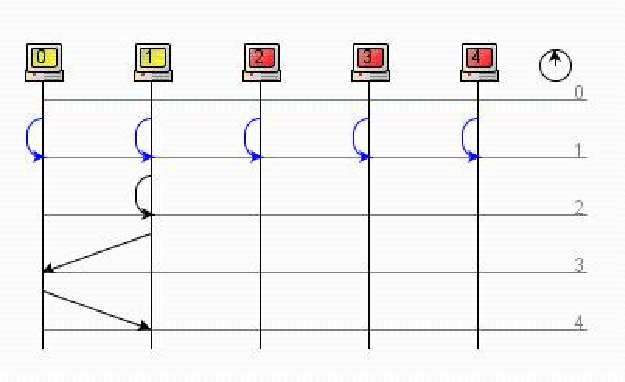
\includegraphics{images/p1ReadSeq.pdf}
    \caption{Daten, die nicht durch eine Ursprungsgerade separabel sind.}
    \label{fig-nichtseparierbar}
\end{figure}

\noindent
Dies erreicht man mit einer sogenannten \textbf{bias unit}.
Das Bias-Gewicht\footnote{
    vgl. [RN09:839]
} ist ein Wert, der zu der Gleichung aus Definition\ref{eq:gl-rpact} hinzuaddiert wird, und für eine Verschiebung der Ursprungsgeraden\footnote{
    im $ \mathbb{R}^n$ durch eine Hyperebene im Ursprung~\cite[215]{Ert21a}
} sorgt.

Den Eingabedaten wird ein fester Eingabewert $x_{n+1} = 1$ hinzufügt: Der Eingabevektor $x \in  \mathbb{R}^n$ wird \textit{erweitert}: $(x_1, ..., x_n, 1)$ (vgl.~\cite[58]{Roj93}).

\noindent
Der bias $b$ wird für unser Beispiel im $ \mathbb{R}^2$ mit Definition\ref{eq:gl-rpact} in die Berechnung Schwellenwerts miteinbezogen:

\begin{equation}
P(x) = \begin{cases}
            1 &\text{falls} &wx > 0 \\
            0 &\text{sonst}
\end{cases}
\end{equation}

\noindent
wobei

\begin{equation}
wx = b + \sum^n_{i=1} w_ix_i
\label{eq:gl-net}
\end{equation}

\noindent
Die Gleichung für die Trenngerade für unser Beispiel im $\mathbb{R}^2$ lautet somit

\begin{equation}
b + w_1x_1 + w_2x_2 = 0
\end{equation}

\noindent
Wenn wir $b$ auf die rechte Seite der Gleichung bringen, kann $b$ auch als Schwellenwert $\Theta = -b$ betrachtet werden:

\begin{equation}
w_1x_1 + w_2x_2 = \Theta
\end{equation}

\noindent
Für unser $x_2$ im $ \mathbb{R}^2$ folgt dann insgesamt mit $w_2 = 1$ und $x_1 = 0$:

\begin{equation}
x_2 = \Theta/w_2 -(w_1/w_2)x_1  = \Theta
\end{equation}

\noindent
was der Abstand $x_2$ von der $y$-Achse ist.

\noindent
Mit $b$ als Teil der Eingabe folgt auch dessen Gewichtung $bw_{n+1} = w_{n+1}$.
Mit $0$ als Schwellenwert wird dadurch eine Verschiebung der Trenngeraden entlang der $y$-Achse im $ \mathbb{R}^2$ bzw. eine Verschiebung der Hyperebene im $ \mathbb{R}^n$ ermöglicht~\cite[215]{Ert21a} \footnote{
    einen Überblick über die geometrischen Zusammenhänge liefert ``Einführung in die Neuroinformatik`` von Prof. Dr. G. Sommer \url{https://www.informatik.uni-kiel.de/inf/Sommer/doc/Downloads/Skripte/neuroskript.pdf}:33 ff. (abgerufen 27.08.2023)
}.

\begin{figure}[h]
    \centering
    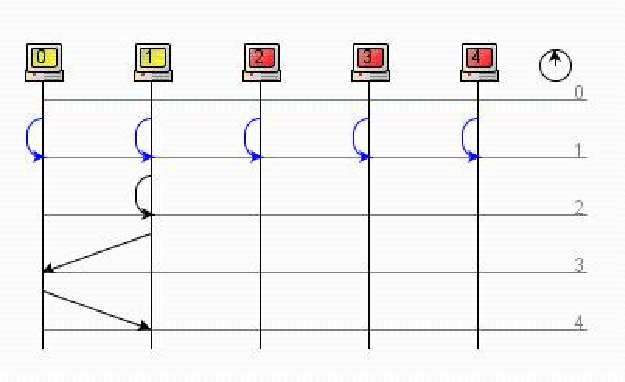
\includegraphics{images/p1ReadSeq.pdf}
    \caption{Geometrische Interpretation der Perzeptron-Funktion im $\mathbb{R}^2$}
    \label{fig-geominterpretation}
\end{figure}

\noindent\fbox{%
    \parbox{\textwidth}{%
        Eine Implementierung eines Rosenblatt-Perzeptrons in Python findet sich in \ref{appendix:pythonperzeptron}.
    }%
}




\subsection{Die XOR-Funktion}

Wenn ein Perzeptron nicht konvergiert, kann es ausreichen, die Anzahl der Epochen zu erhöhen, damit ein passender Gewichtsvektor gefunden wird\footnote{
    \textit{Arbib et al} berufen sich auf das Konvergenz-Theorem und führen an, dass ``[das Rosenblatt Perzeptron] does not yield an endless seesaw, but will eventually converge to a correct set of weights if one exists, albeit perhaps after many iterations through the set of trial patterns.``~\cite[20]{Arb03}: \textit{Minsky und Papert} formulieren lose: ``if the sets are separable [...], then the program will separate them``~\cite[165]{MP88} und stellen im Hinblick auf Parameteranpassungen fest: ``Usually, when a failure occurred, neither prolonging the training experiments nor building larger machines helped.``~\cite[xi]{MP88}
}.

\begin{figure}[h]
    \centering
    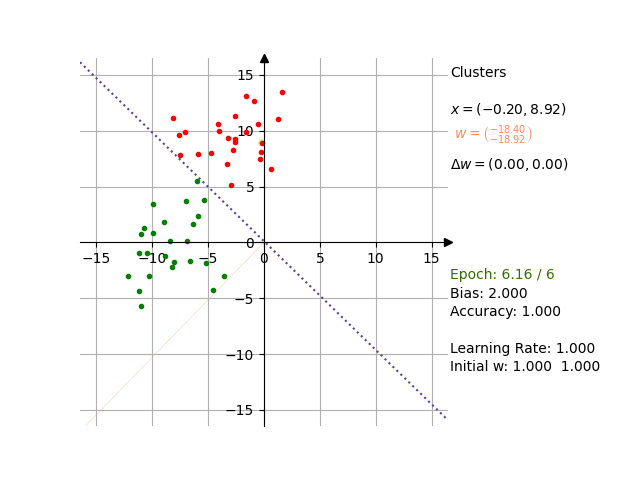
\includegraphics{images/rosenblatt/blob_success.png}
    \caption{}
    \label{fig-rp-blobs}
    \small Ein Perzeptron wird mit einer großen Datenmengen (50 Einträg) trainiert. Nach knapp 300 Trainingsschritten (in der 6ten Epoche) wird die Trenngerade gefunden. (Quelle: eigene)
\end{figure}

\noindent
Allerdings kann es bereits bei wenigen Daten und beliebig großer Epochenzahl passieren, dass ein Perzeptron nicht konvergiert, nämlich wenn die Daten nicht linear separabel sind~\cite[20]{Arb03}.

Als Beispiel betrachten wir die boolesche Funktion \textbf{XOR} (vgl. Tabelle~\ref{tab:xor}). In Abbildung~\ref{fig-rp-xor } ist die geometrische Repräsentation der möglichen Interpretationen für $A \oplus B$ dargestellt.
Zwar lassen sich die Elemente separieren, aber nicht linear.
Es müßte sonst ein $w_1, w_2$ existieren, das folgende Ungleichungen erfüllt:\\


$w_10 + w_20 < \Theta$\\

$w_11 + w_20 \geq \Theta \implies w_1 \geq \Theta$\\

$w_10 + w_21 \geq \Theta \implies w_2 \geq \Theta$\\

$w_11 + w_21 < \Theta$\\

\noindent
Offensichtlich kann $w_1 + w_2 < \Theta$ nicht erfüllt werden, wenn gleichzeitig $w_1 \geq \Theta$ und $w_2 \geq \Theta$ gilt.

\begin{figure}[h]
    \centering
    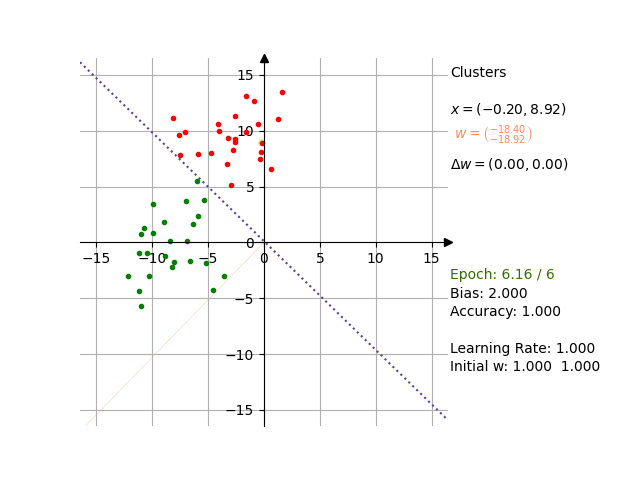
\includegraphics{images/rosenblatt/blob_success.png}
    \caption{Interpretationen der XOR-Funktion im kartesischen Koordinatensystem. Eine lineare Trenngerade existiert für die Werte nicht.}
    \label{fig-rp-xor}
\end{figure}

\subsection{Der KI-Winter}\label{kiwinter}

In \textit{Perceptrons - An introduction to Computational Geometry (1969)}~\cite{MP88} behandeln \textit{Minsky und Papert} u.a. das Verhalten des Perzeptrons im Fall nicht-separabler Daten\footnote{
    in~\cite[181 ff.]{MP88}
} sowie das Problem bzgl. \textit{recognition of connectedness}\footnote{
    s. \cite[12, ``Theorem 0.8``]{MP88} sowie~\cite[249 f.]{MP88}. In dem Epilog, der 19 Jahre später in einer Neuausgabe von \textit{Minsky und Papert} veröffentlicht wird, machen sie deutlich, dass sie damit nicht nachweisen wollten, dass ein Perzeptron nicht in der Lage zu der Erkennung zusammenhängender geometrischer Figuren sei, sondern dass die Komplexität von verschiedenen Aufgaben Anforderungen an ein Perzeptron stellt, die zu der damaligen Zeit (Ende 1950er / Anfang 1960er) schwierig umzusetzen gewesen sind (vgl. ~\cite[250]{MP88})
}, bei dem es um die Erkennung zusammenhängender geometrischer Figuren geht.
Ihr Anliegen mit dem Buch ist es, die (mathematischen) Grenzen des Rosenblatt-Perzeptrons auf ein formales Gerüst zu stellen (vgl.~\cite[249]{MP88}).
Ihre Ausführungen verstärken aber die ohnehin schon skeptische Haltung\footnote{
    Here was a machine that could do pattern recognition in a humanlike way; it could recognize all kinds of things. Almost everyone at MIT was very skeptical``~\cite[99]{AR98}
} gegenüber der Fähigkeiten des Perzeptrons\footnote{
    auch wegen schlechter Skalierbarkeit des Modells in der Praxis~\cite[159]{AR88}
} und künstlicher neuronaler Netze allgemein, was \textit{Anderson und Rosenfeld} rückblickend auch auf Aussagen in der Einleitung des Buches zurückführen wie

\blockquote[{~\cite[19]{MP88}}]{
hundreds of projects and experiments [bzgl. des Perzeptrons] were generally disappointing, and the explanations inconclusive. The machines usually work quite well on very simple problems but detoriate very rapidly as the tasks assigned to the get harder.
}

\noindent
Auch eine generelle Irritation und Enttäuschung über das Perzeptron-Modell meinen \textit{Anderson und Rosenfeld} zu erkennen:

\blockquote[{~\cite[232]{MP88}}]{
we [Minsky und Papert] consider it to be an important research problem to elucidate (or reject) our intuitive judgement that the extension is sterile.
}

\noindent
Diesen ``Pessimismus`` betrachten \textit{Minsky und Papert} im Jahr 1988 in Retrospektive (s. ~\cite[xiii]{MP88}). Sie sind sich der Behauptung bewusst, ihr Buch hätte mit dem Aufzeigen der Grenzen des Rosenblatt-Modells den Forscherdrang an maschinellem Lernen gebremst:

\blockquote[{~\cite[xii]{MP88}}]{
One popular version is  that the publication of our book so discouraged research on learning in network machines that a promising line of research was interrupted.
}

\noindent
\textit{Anderson und Rosenfeld} erwähnen ``the influence of Marvin Minsky and Seymour Papert on the loss of interest in neural networks during the 1970s``~\cite[X]{AR98}, worüber ihre Interviewpartner in gleicher Quelle sprechen.

\textit{Russell und Norvig} fassen zusammen, dass \textit{Minsky und Papert} in ihrem Buch bewiesen haben, dass ein Perzeptron alles lernen kann, was es auch darstellen kann, aber es könnte halt nur sehr wenig darstellen[RN09:45]\footnote{
    vgl. hierzu~\cite[xiii]{MP88}
}. Auf gleicher Seite verweisen sie auf die zunehmende Komplexität der zu berechnenden Modelle, die nicht alleine durch schnellere und bessere Hardware kompensiert werden konnte.

Der Lighthill Report\footnote{
    ``Workers entered the field around 1950, and even around 1960, with high hopes that are very far from having been realised in 1972. In no part of the field have the discoveries made so far produced the major impact that was then promised.`` in \url{https://www.chilton-computing.org.uk/inf/literature/reports/lighthill\_report/p001.htm}, ``3 Past disappointments``, abgerufen 28.08.2023
} sollte dann 1973 eine Grundlage für die Entscheidung der britischen Regierung darstellen, das Budget für die Forschung an KI zu kürzen [RN09:45]. Neuronale Netze wurden als Grundlage künstlicher Intelligenz zunächst verworfen\footnote{
    vgl.~\cite[641]{Ola96}
}, und die Forschung daran ging zurück, bis sie Anfang/Mitte der 1980er Jahre wieder aufgenommen wurde: Diese Periode ist gemeinhin als ``KI-Winter`` (vgl. \ref{appendix:kiwinter}) bekannt.

